\chapter{Theoretische und technische Grundlagen}

Im Rahmen dieses Kapitels werden die maßgeblichen Technologien und Konzepte dargelegt, auf denen das entwickelte Modell basiert. Der Fokus liegt auf der automatisierten Objekterkennung, Textextraktion und strukturierten Informationsverarbeitung aus Gleisplänen.
\section{Grafische Gleispläne im Bahnkontext}
Die Modellierung eines Bahnhofs stellt eine komplexe Aufgabe dar, da ein solcher in der Regel aus Hunderten von Gleisen und Weichen sowie zahlreichen Signalen besteht. 
Die manuelle Erstellung eines Bahnhofsmodells, das den physischen Details eines Bahnhofs entspricht, erfordert in der Regel mehrere Wochen Arbeit. Dies hat signifikante 
Auswirkungen auf die Anwendbarkeit und den Umfang vieler Methoden.\cite{railroadstationdrawing}

\subsection{Grundlagen des Gleisplans}
Der Gleisplan bildet die fundamentale Datengrundlage für die Planung, den Bau und den operativen Betrieb von Bahnanlagen. Er repräsentiert die technische Infrastruktur und dient als visuelle Schnittstelle zwischen der physischen Außenanlage und der sicherungstechnischen Logik (Stellwerk).
\\
Gleispläne existieren in zwei Darstellungsformen \cite{Pachl}: maßstäbliche 
Lagepläne (topografisch, bautechnisch) und schematische Übersichtspläne 
(topologisch, sicherungstechnisch). Diese Arbeit fokussiert letztere, da sie 
die logischen Fahrwegbeziehungen priorisieren und die Grundlage für die Stellwerksplanung bilden.

Gleispläne enthalten drei Symbolkategorien: (1) Fahrwegelemente (Gleise, Weichen), 
(2) Sicherungstechnik (Signale, Achszähler), (3) Metadaten (Bezeichner, 
Kilometrierung). Jedes Element trägt eindeutige Labels zur Identifikation.

Obwohl diese Pläne in der heutigen Ingenieurspraxis mittels CAD-Systemen (Computer Aided Design) erstellt werden, liegt die primäre Herausforderung für eine automatisierte Auswertung nicht im Dateiformat, sondern in der korrekten semantischen Interpretation dieser abstrahierten Symbolik und ihrer logischen Verknüpfung \cite{Pachl}.

\begin{figure}[h]
    \centering
    \includegraphics[width=1\textwidth]{images/gleisplandrawio.png} 
    \caption{Ausschnitt eines schematischen Gleisplans mit Darstellung von Signalen, Weichen und Gleisbezeichnungen (Beispielhafte Darstellung) aus Quelle \cite{railroadstationdrawing}}
    \label{fig:gleisplan_schema}
\end{figure}

\subsection{Bahntechnische Symbole und ihre Klassifikation}
\label{sec:Bahntechnischesymbole}
In den Gleisplänen kommen zahlreiche Symbole zum Einsatz, um die verschiedenen technischen Objekte, Anlagenkomponenten und zusätzlichen Informationen übersichtlich darzustellen. Diese Symboldarstellung dient nicht nur der Visualisierung der Gleiskomponenten, sondern bildet auch die Grundlage für Planung, Projektierung, Dokumentation und spätere Anwendung. \cite{signallayout} Da der Gleisplan eine zentrale Schnittstelle zwischen technischer Planung, 
betrieblicher Umsetzung und sicherheitstechnischen Systemen darstellt, ist eine präzise, klare und einheitliche Symbolklassifizierung notwendig. Die für diese Arbeit relevanten Symbolklassen gliedern sich in drei funktionale 
Kategorien (siehe Tabelle \ref{tab:symbol_categories}):

\begin{table}[h]
\centering
\begin{tabular}{|p{3cm}|p{12cm}|}
\hline
\textbf{Kategorie} & \textbf{Elemente und Funktion} \\
\hline
Infrastruktur & \textbf{Signale}: Fahrterlaubnis und Geschwindigkeitsvorgabe. 
\textbf{Weichen}: Fahrwegverzweigungen. \textbf{Isolierstöße}: Elektrische 
Gleistrennung. \textbf{Achszähler}: Belegungserkennung. \\
\hline
Zugbeeinflussung & \textbf{Balisen}: Punktförmige Datenübertragung an Zug. 
\textbf{Gleismagnete}: Induktive Informationsübertragung. \textbf{Gleiskoppelspulen}: 
Elektromagnetische Kopplung. \\
\hline
Metadaten & \textbf{Positionsangaben}: Kilometrierung, Lagepunkte. 
\textbf{Gleisabschnittsnamen}: Eindeutige Gleisidentifikation. \\
\hline
\end{tabular}
\caption{Klassifikation bahntechnischer Symbole}
\label{tab:symbol_categories}
\end{table}

Die detaillierte visuelle Darstellung dieser Symbole erfolgt in Abschnitt 4.1.
\section{Grundlagen der Objekterkennung mit Deep Learning}


Die Objekterkennung stellt ein zentrales Forschungsgebiet im Bereich der Computer Vision dar. Das Ziel besteht darin, in einem Bild nicht nur die Klassifizierung vorhandener Objekte zu erreichen, sondern auch die 
Lokalisierung dieser Positionen in Form von Bounding Boxes. In der vorliegenden Arbeit wird die Objekterkennung primär zur automatisierten Analyse von Symbolen und Positionsinformationen in Gleisplänen eingesetzt. 
In den letzten Jahren haben sich Deep-Learning-basierte Verfahren, insbesondere Convolutional Neural Networks (CNNs), als Standard etabliert. In Bezug auf erkennungsbasierte Aufgaben haben 
sich die Architekturen YOLO, Faster R-CNN, SSD sowie die neuen Varianten DETR und RTMDet als besonders sinnvoll erwiesen. Da die Gleispläne neben Symbolen auch Textinformationen wie Signalnamen, Positionen, Gleisstromkreisnamen usw. enthalten, 
werden für diese Zwecke zusätzlich optische Zeichenerkennungsverfahren (OCR) eingesetzt. OCR Verfahren (Optical Character Recognition), zu denen beispielsweise Tesseract oder EasyOCR zählen, sind dazu fähig, Textelemente automatisch zu lesen und zu extrahieren. 
Daher wird die visuelle Objekterkennung durch OCR unterstützt und es kommt zur vollständigen semantischen Erfassung der Pläne.

\subsection{Computer Vision}

Computer Vision bezeichnet die automatische Extraktion und Interpretation visueller 
Information aus Bildern und Videos \cite{szeliski2022}. Moderne Ansätze basieren auf 
Deep Learning (insbesondere CNNs), das deutlich robuster gegenüber Rauschen, 
Verzerrungen und komplexen Layouts ist als regelbasierte Verfahren \cite{helle2023}.

In dieser Arbeit wird Computer Vision zur automatisierten Analyse von Gleisplänen 
eingesetzt: Symbolerkennung (YOLO) und Texterkennung (OCR) transformieren 
unstrukturierte Pläne in maschinenlesbare Datenstrukturen.

\subsection{Neuronale Netze und Convolutional Neural Networks (CNNs)}


Convolutional Neural Networks bilden die methodische Grundlage moderner 
Objekterkennungssysteme. Ihre Architektur besteht aus hierarchischen Schichten:
Convolutional Layers extrahieren lokale Merkmale (Kanten, Texturen), Pooling 
Layers reduzieren die Dimensionalität, und Fully Connected Layers führen die 
finale Klassifikation durch \cite{Wang2022Classification}.

Für die vorliegende Arbeit ist insbesondere die Anwendung dieser Prinzipien 
in der YOLOv8-Architektur relevant (vgl. Abschnitt 3.2.4), die eine einstufige 
Objekterkennung mit hoher Echtzeitfähigkeit ermöglicht.



\subsection{Training und Generalisierung}

CNNs erfordern große annotierte Datensätze für robustes Training. Bei 
kundenspezifischen Gleisplänen ist dies eine Herausforderung (Domain Shift 
\cite{NIPS2014_532a2f85}). Zwei Ansätze adressieren dies:

\begin{itemize}
    \item \textbf{Transfer Learning}: Verwendung vortrainierter Modelle (z.B. YOLOv8 
    auf COCO) mit Feinabstimmung auf Gleisplan-Daten \cite{transferlearning}.
    \item \textbf{Data Augmentation}: Künstliche Datensatzerweiterung durch Rotationen, 
    Skalierungen, Helligkeitsanpassungen \cite{dataugmentation}.
\end{itemize}

Die praktische Umsetzung wird in Kapitel 6.2 beschrieben, die Evaluierung der 
Generalisierung in Kapitel 7.2.


\subsection{YOLOv8 - Ein modernes Framework für Echtzeit-Objekterkennung}

You Only Look Once Version 8 (YOLOv8) stellt eine spezifische Architektur dar, die auf der Grundlage von Faltungsneuronalen Netzen entwickelt wurde. Während konventionelle CNNs für die Bildklassifizierung zum Einsatz kommen, erweitert YOLOv8 diesen Ansatz, indem die Klassifizierung und Lokalisierung von Objekten in einem einzigen Schritt erfolgt.\cite{RCNN} Diese Eigenschaft unterscheidet YOLOv8 von zweistufigen Prozessen wie Faster R-CNN, bei denen zunächst die Regionsvorschläge erstellt und anschließend klassifiziert werden. 
Die einstufige Architektur des YOLOv8 ermöglicht eine signifikante Beschleunigung ohne signifikante Einbußen bei der Genauigkeit. \cite{redmon2016lookonceunifiedrealtime}
\\
\\
Die YOLOv8-Architektur gliedert sich in folgende drei funktionale Komponenten:
\begin{table}[ht]
\centering
\begin{tabular}{|p{2.5cm}|p{9cm}|}
    \hline
    \textbf{Komponente} & \textbf{Beschreibung}  \\
    \hline
    Backbone & Extrahiert hierarchische Merkmale (CSPDarknet, MobileNet, EfficientNet)  \\
    \hline
    Neck & Aggregiert Features auf verschiedenen Skalen (FPN, PAN, BiFPN)  \\
    \hline
    Head & Führt Bounding-Box-Regression und Klassifikation durch (anchor-free)  \\
    \hline
\end{tabular}
\caption{Hauptkomponenten der YOLOv8 Architektur}
\label{tab:komponenten}
\end{table}

Das Backbone übernimmt die Aufgaben der hierarchischen Merkmalsextraktion, wie sie auch in klassischen CNNs ausgeführt werden, wobei moderne Varianten wie CSPdarknet oder EfficientNet zum Einsatz kommen können. 
Der Neck aggregiert die Merkmale aus verschiedenen Ebenen und gewährleistet somit eine zuverlässige Erkennung sowohl kleiner als auch großer Objekte. Schließlich wird durch den Head die eigentliche Bounding-Box-Regression sowie die Klassifizierung der erkannten Symbole durchgeführt.  Charakteristisch für YOLOv8 ist die Anchor-free Architektur, die die Komplexität der Bounding-Box-Berechnung reduziert und die Generalisierung erhöht. \cite{yaseen2024yolov8indepthexplorationinternal}
\\
\\
Im Vergleich zu den älteren Versionen (beispielsweise YOLOv5 oder YOLOv7) zeichnet sich YOLOv8 durch eine verbesserte Trainingsstabilität, tiefere Backbone-Netzwerke und die native Unterstützung für zusätzliche Aufgaben wie Segmentierung oder Pose Estimation aus. Diese Erweiterungen resultieren in einer hohen Flexibilität und eignen sich daher insbesondere für komplexe Anwendungsbereiche, wie etwa die Analyse großformatiger Gleispläne.\cite{yolov8_ultralytics}
\\
\\
Darüber hinaus sind weitere Versionen, wie etwa YOLOv9 (2024) und YOLOv10 (2025), mit spezifischen Optimierungen ausgestattet, die sich auf die Effizienz und Genauigkeit fokussieren. In der neuesten Version von YOLOv9 wurde ein neues Feature-Extraktionsmodul integriert, das den Namen \enquote{Programmable Gradient Information Bottleneck} trägt. Dieses Modul dient dazu, das Gleichgewicht zwischen Genauigkeit und Modellkomplexität zu verbessern.\cite{wang2024yolov9learningwantlearn}
Im Gegensatz dazu optimiert YOLOv10 die Architektur zusätzlich im Hinblick auf ein effizientes Training und Inferenz, wodurch es sich besser für mobile oder eingebettete Systeme eignet.\cite{wang2024yolov10realtimeendtoendobject}
\\
\\
Für die Erstellung der Masterarbeit wurde YOLOv8 ausgewählt, da es zum Zeitpunkt der Entwicklung eine stabile, umfassend dokumentierte und sowohl in der Forschung als auch in der Industrie etablierte Version darstellte. Darüber hinaus bietet YOLOv8 bereits alle relevanten Funktionen für die Objekterkennung in Gleispläne, insbesondere in der anchor-free Architektur, die Unterstützung verschiedener Backbone-Varianten sowie die Möglichkeit zur Erweiterung auf Segmentierungs- und Klassifizierungsaufgaben. 
Neuere Versionen gehen mit einer Reihe von Verbesserungen einher, wobei die Vorteile jedoch hauptsächlich in den spezifischen Anwendungen liegen, die den Fokus dieser Arbeit bilden.


\subsection{Abgrenzung zu Alternativen}

Alternative Architekturen wie Faster R-CNN (höhere Genauigkeit, aber zu langsam 
für große Gleispläne), SSD (schnell, aber ungenau bei kleinen Symbolen) und 
RTMDet (interessant für rotierte Objekte, aber weniger etabliert) wurden evaluiert. 
Tabelle \ref{tab:detektor-vergleich} fasst die Bewertung zusammen. YOLOv8 bietet 
die optimale Balance aus Geschwindigkeit, Genauigkeit und Community-Support für 
diese Anwendung \cite{yolov8_ultralytics}.

\begin{table}[H]
\centering
\renewcommand{\arraystretch}{1.3} % mehr Zeilenhöhe
\begin{tabularx}{\textwidth}{|p{2.2cm}|p{2.2cm}|Y|Y|Y|}
\hline
\textbf{Architektur} & \textbf{Typ / Ansatz} & \textbf{Stärken} & \textbf{Schwächen} & \textbf{Eignung für diese Arbeit} \\
\hline
\textbf{Faster R-CNN} & Two-Stage-Detektor & Sehr hohe Genauigkeit, gute Erkennung auch bei komplexen Szenen & Sehr rechenintensiv, geringe Geschwindigkeit, ungeeignet für Echtzeit & (zu langsam für große Gleispläne) \\
\hline
\textbf{SSD} & Single-Stage-Detektor & Schnell, effizient, weniger rechenintensiv & Geringere Genauigkeit bei kleinen und dichten Objekten &  (ungenau bei kleinen Symbolen) \\
\hline
\textbf{RTMDet} & Single-Stage (rotation-aware) & Robust bei geneigten oder verdrehten Symbolen, gute Echtzeitleistung & Weniger etabliert, geringere Verfügbarkeit an Tools und Frameworks &  (interessant, aber weniger stabil) \\
\hline
\textbf{YOLOv8} & Single-Stage-Detektor & Sehr gute Balance aus Geschwindigkeit und Genauigkeit, moderne Architektur (Backbone/Neck/Head), breite Community-Unterstützung, Zusatzaufgaben (Segmentierung, Pose) & Höherer Hardwarebedarf als SSD, relativ neu (weniger Langzeitstudien) & (optimale Wahl für Prototyp) \\
\hline
\end{tabularx}
\caption{Vergleich verschiedener Architekturen}
\label{tab:detektor-vergleich}
\end{table}

\section{YOLOv8obb - Architektur und Grundlagen der orientierten Objekterkennung}
Die präzise Erfassung von Objekten in technischen Zeichnungen erfordert Methoden, die über die klassische Erkennung mit Hilfe von parallelen Achsenrechtecken (Axis-Aligned Bounding Boxes, AABB) hinausgehen. Dieser Abschnitt führt das Konzept der orientierten Begrenzungsrahmen (OBB) ein und erklärt die Architektur des YOLOobb-Modells, das später in der Masterarbeit verwendet wird.


\subsection{Metriken und Filterung: IoU und NMS}

Die \textbf{Intersection over Union (IoU)} quantifiziert Bounding-Box-Überlappung:

$$\text{IoU}(A,B) = \frac{|A \cap B|}{|A \cup B|}$$

\textbf{Non Maximum Suppression (NMS)} eliminiert redundante Detektionen: Iterativ 
wird die konfidenteste Box gewählt und alle Boxen mit IoU > Schwellenwert unterdrückt.

Bei achsenparallelen Boxen (AABB) führt NMS in dichten Layouts zu Fehlunterdrückungen, 
da geometrisch getrennte, aber axial überlappende Objekte fälschlich als Duplikate 
erkannt werden. Orientierte Bounding Boxes (OBB) mit rotierter IoU lösen dieses 
Problem \cite{yolov8_ultralytics}.



\subsection{Repräsentationsformen der Objecterkennung: AABB vs OBB}
Die Wahl der Darstellung für die Lokalisierung der Objekte ist eine grundlegende Entscheidung beim Entwurf eines Detektionssystems.\cite{yolov8_ultralytics} Ein Begrenzungsrahmen (Bounding Box) beschreibt die räumliche Ausdehnung und die Position eines Objekts und dient als Grundlage für das Training (Box-Regression), die Bewertung (Intersection over Union) und auch die Nachbearbeitung (Non Maximum Suppression). In der Praxis haben sich zwei Hauptansätze etabliert: achsenparallele Begrenzungsrahmen (AABB) und orientierte Begrenzungsrahmen (OBB).

\begin{enumerate}
    \item \textbf{Achsenparallele Bounding Boxes (AABB)} - Die am weitesten verbreitete Form in klassischen Detektoren (wie Faster R-CNN, Standard YOLO) ist das achsparallel ausgerichtete Rechteck, dessen Kanten parallel zur Bildachse verlaufen. Formal wird AABB meist über die Koordinaten der oberen linken und unteren rechten Kanten ($x_min,y_min,x_max,y_max$) oder über das Zentrum sowie die Breite und Höhe ($c_x, c_y, w, h$) definiert.
    \begin{itemize}
        \item Vorteile - Die Berechnung der geometrischen Operationen, insbesondere der Schnittflächen für den Intersection over Union (IoU), ist trivial und recheneffizient. Dies ermöglicht sehr schnelle Trainings- und Inferenzzeiten.
        \item Nachteile - AABBs approximieren die Form eines schräg oder diagonal verlaufenden Objekts nur unzureichend. Bei einem gedrehten Textfeld umschließt eine AABB unvermeidlich eine große Fläche des Hintergrunds („Leerraum“). Außerdem führt die achsparallele Projektion zu massiven Überlappungen mit den nahegelegenen Objekten in dicht gepackten Szenen. Dies erschwert die Trennung jeder einzelnen Instanz.
    \end{itemize}
    \item \textbf{Orientierte Bounding Boxes (OBB)} - Um die Einschränkungen von AABBs zu überwinden, verwenden moderne Ansätze insbesondere in der Fernerkundung und der Szenentexterkennung orientierte Begrenzungsboxen.Im Vergleich zu  AABBs beschreiben die Oriented  Bounding Boxes ein Objekt durch eine gedrehte rechteckige Überlagerung, die zur geometrischen Hauptachse des Objekts geneigt ist. Die OBB verwenden eine Formel, die durch 5-Tupel definiert ist:

    $$OBB = (c_x,c_y, w, h,\theta)$$

    Hier stellen die ($c_x,c_y$) das Zentrum der Box dar, $(w,h)$ die Dehnung entlang der lokalen Achse und auch $\theta$, das den Rotationswinkel relativ zur horizontalen Bildachse repräsentiert. Da die unterschiedliche Parametrisierung (z. B. der Austausch von w und h bei einer Drehung um 90°) dieselben geometrischen Objekte beschreiben kann, verwenden die modernen Implementierungen normalisierte Darstellungen oder periodische Verlustfunktionen (kreisförmige glatte Labels), um numerische Instabilitäten während des Trainings zu vermeiden.
    \begin{itemize}
        \item Vorteile - OBBs passen sich an die Hauptachse des Objekts an. Dadurch wird der Hintergrundanteil innerhalb der Box erheblich minimiert, was für nachgelagerte Klassifizierungsaufgaben (wie OCR) sehr vorteilhaft ist, da weniger Störsignale („Noise“) verarbeitet werden müssen. Darüber hinaus liefert der Winkel 	$\theta$ intrinsische Informationen über die Richtung, die für die geometrische Entzerrung (Rectification) verwendet werden können.
        \item Nachteile - Die Einführung des Winkels erhöht die Komplexität der Verlustfunktion und der Metriken. Daher muss die rotierte IoU als die Schnittfläche zwischen zwei Polygonen berechnet werden, was rechenintensiver ist als bei AABBs.Darüber hinaus erfordert die Periodizität des Winkels (z.B. 0° ~ 360°) spezielle Codierungsstrategien (wie Sinus-Kosinus-Einbettung), um die numerische Stabilität während des Trainings zu gewährleisten.
    \end{itemize}

\end{enumerate}
\begin{figure}[H]
\centering
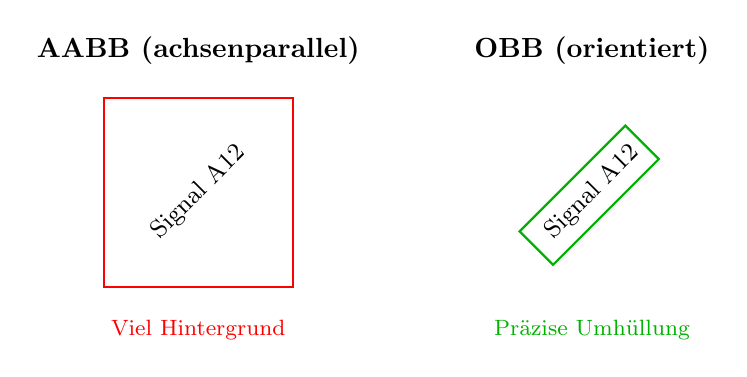
\begin{tikzpicture}[scale=1.0]
    % LEFT: AABB
    \begin{scope}
        \node[above, font=\bfseries] at (1.5, 3) {AABB (achsenparallel)};
        
        % Rotated text (45 degrees)
        \node[rotate=45, font=\small] at (1.5, 1.5) {Signal A12};
        
        % Horizontal bounding box (AABB) - contains lots of background
        \draw[thick, red] (0.3, 0.3) rectangle (2.7, 2.7);
        
        % Annotation
        \node[below, font=\footnotesize, red] at (1.5, 0) {Viel Hintergrund};
    \end{scope}
    
    % RIGHT: OBB
    \begin{scope}[xshift=5cm]
        \node[above, font=\bfseries] at (1.5, 3) {OBB (orientiert)};
        
        % Rotated text (45 degrees)
        \node[rotate=45, font=\small] at (1.5, 1.5) {Signal A12};
        
        % Oriented bounding box (OBB) - tight fit
        \draw[thick, green!70!black, rotate around={45:(1.5,1.5)}] 
            (0.5, 1.2) rectangle (2.4, 1.8);
        
        % Annotation
        \node[below, font=\footnotesize, green!70!black] at (1.5, 0) 
            {Präzise Umhüllung};
    \end{scope}
\end{tikzpicture}
\caption{Vergleich zwischen achsenparalleler Bounding Box (AABB, rot) und 
orientierter Bounding Box (OBB, grün) bei rotiertem Text: OBB minimiert 
Hintergrundfläche und reduziert Überlappungen mit Nachbarobjekten}
\label{fig:aabb_vs_obb}
\end{figure}
\subsection{YOLOv8obb Architektur und Modellgrößen}
Die orientierte Objekterkennung mit YOLOv8-OBB erweitert die klassische achsparallele Objekterkennung durch die explizite Schätzung eines Rotationswinkels ($\theta$) für jedes Objekt. In Anordnungen mit kleinen, teilweise geneigten Symbolen und dicht gedrängten liegenden Texten führt dies zu einer deutlich höheren Lokalisierungsgenauigkeit und liefert zusätzliche Orientierungsinformationen, die in nachgelagerten Schritten, insbesondere für die OCR-Normalisierung und semantische Verknüpfung, genutzt werden können.

YOLOv8 ist ein einstufiger, ankerfreier Detektor. Anstatt vordefinierter Ankerpunkte werden die Boxen direkt auf zukünftige Positionen regressiert, was den Trainingsprozess stabilisiert, die Hyperparameter reduziert und die Laufzeiteffizienz erhöht. Seine Architektur kann durch die folgenden Teile beschrieben werden:

\begin{enumerate}
    \item \textbf{Backbone}: Der C2f-Block, eine Weiterentwicklung des CSP/C4, erhöht die Repräsentationsfähigkeit bei moderatem Rechenaufwand. Die Breite (Kanäle) und die Tiefe (Schichten) werden je nach Modellgröße skaliert.
    \item \textbf{Neck}: Ein FPN/PAN-ähnlicher Neck fusioniert die Merkmale über die Skalen hinweg, um sehr kleine (z.\,B. feine Symbole, Kennplatten) bis hin zu größeren Objekten robust zu unterstützen.
    \item \textbf{Decoupled Head}: Getrennte Pfade für Klassifikation und Box-Regression stabilisieren das Training. In den OBB-Varianten regressiert der Head neben ($c_x, c_y, w, h$) zusätzlich den Orientierungswinkel $\theta$ (insgesamt 5 Parameter für die Box).
    \item \textbf{Winkelkodierung und Normalisierung}: Aufgrund der Periodizität von Theta (äquivalente Darstellungen mit $\pm\theta$ bei Austausch von $w/h$) normalisieren die Implementierungen die Darstellungen in einem kanonischen Bereich. In der Literatur können direkte Winkelregressionen oder Sinus/Cosinus-Codes verwendet werden, um Diskontinuitäten zu vermeiden und die Konvergenz zu stabilisieren (vergleichbar mit MMRotate, Oriented R-CNN).
\end{enumerate}

\textbf{Rotation Aware Losses und Filterung}
\begin{itemize}
    \item Box-Regression Loss: In OBB-Head werden spezielle rotationsbewusste Verlustfunktionen verwendet, die auf die Drehung der Boxen abgestimmt sind. Sie basieren entweder auf dem rotierten IoU (rIoU), der Gaußschen Wasserstein-Distanz (GWD) oder den auf der Kullback-Leibler-Divergenz (KLD) basierenden Verlusten. Solche Distanzmetriken behandeln die Boxen als Gaußsche Verteilungen und führen zu einer stabilen und robusten Regression des Winkels, insbesondere bei komplexen Orientierungen in den Plänen.
    \item Repräsentation Normalisierung: Implementierungen normalisieren den OBB-Parameter in einem kanonischen Winkelbereich, z. B. [0,90), um die Gleichwertigkeit verschiedener Darstellungen zu eliminieren (z. B. w/h Tausch bei 0 bzw. ±90°) und die Regression zu stabilisieren.
    \item Rotated NMS (rNMS): Rotierte NMS (rNMS): Die endgültige Filterung der Detektionsergebnisse muss über rotierte Non-Maximum-Suppression (rNMS) erfolgen. Nur die rNMS berücksichtigt die tatsächliche Überlappung der rotierten Boxen (rIoU), was grundlegend für die korrekte Trennung dicht liegender Nachbarobjekte in den Gleisplan-Patches ist.
\end{itemize}

\textbf{Modellgrößen und Auswahlkriterien}
YOLOv8 wird in mehreren Skalierungsvarianten (n, s, m, l, x) angeboten. Diese unterscheiden sich durch Breiten- und Tiefenmultiplikatoren (Breiten-/Tiefenskalierung) und stellen einen Kompromiss zwischen Genauigkeit der Erkennung, Inferenzlaufzeit und Ressourcenverbrauch dar. Die Eigenschaften von jeder Größe ist unten in Tabelle \ref{tab:Yolov8obbgroßen} 

\begin{table}[ht]
  \centering
  \begin{tabular}{|p{2cm}|p{7cm}|p{5cm}|} % Vertical lines added
    \hline
    \textbf{Variante} & \textbf{Charakteristik} & \textbf{Typische Parameteranzahl (ca.)} \\ \hline
    n (nano) & Sehr leicht, geringste Latenz/Genauigkeit & 3-4 Millionen \\ \hline
    s (small) & Leicht, schnell, für einfache Szenen & 11-12 Millionen \\ \hline
    m (medium) & Ausgewogen für allgemeine Anwendungen & 25-26 Millionen \\ \hline
    l (large) & Größere Kapazität, verbesserte Genauigkeit, für kleine/komplexe Objekte & 43-44 Millionen \\ \hline
    x (extra large) & Höchste Genauigkeit, hoher Ressourcenbedarf & 68-70 Millionen \\ \hline
  \end{tabular}
  \caption{YOLOv8obb Modellgrößen}
  \label{tab:Yolov8obbgroßen}
\end{table}

\textbf{Verwendung im Projektkontext der Masterarbeit} \\
In dieser Arbeit wird die orientierte Objekterkennung zur Analyse sehr großer, hochauflösender technischer Gleispläne eingesetzt. Da die Gesamtbilder die maximal verarbeitbare Eingabegröße des Modells weit überschreiten, werden die Pläne in der Vorverarbeitung in kleine, sich überlappende Bildteile zerlegt. Die Modellauswahl basiert auf dieser spezifischen Methodik:

\begin{itemize}
    \item \textbf{Anforderung an das Modell}: Die Objekte erscheinen innerhalb der kleinen Bildteile als kleine, dichte und rotierte Elemente. Dies erfordert ein Modell mit hoher Kapazität zur präzisen Lokalisierung und Orientierungsbestimmung.
    \item \textbf{Auswahl}: Unter Berücksichtigung der notwendigen höheren Lokalisierungspräzision für kleine, rotierende Symbole und der Anforderung einer praktikablen Inferenzzeit im Offline-Betrieb, wird ein YOLOv8-OBB-Modell der Größenvariante L eingesetzt.
\end{itemize}
Dieser Ansatz stellt sicher, dass die Vorteile der OBB-Darstellung optimal genutzt werden und bildet die Grundlage für die nachfolgende räumliche Analyse und das Zusammenfügen der Ergebnisse (Nachbearbeitung) aus den einzelnen Teilbildern. Angaben zur Datenaufbereitung, den Hyperparametern und der Inferenzstrategie sind in Kapitel 6.2 beschrieben.

\subsection{Evaluationsmetriken für Objekterkennung}

Die Bewertung der Leistung eines Objekterkennungsmodells erfordert standardisierte Metriken, die sowohl die Lokalisierungsgenauigkeit als auch die Klassifikationsgüte quantifizieren.

\subsubsection{Precision, Recall und F1-Score}

Für jede Objektklasse wird die Erkennungsleistung über drei Kernmetriken bewertet:

\begin{itemize}
    \item \textbf{Precision (Präzision)}: Anteil der korrekt erkannten Objekte an 
    allen vorhergesagten Objekten:
    $$\text{Precision} = \frac{TP}{TP + FP}$$
    
    \item \textbf{Recall (Trefferquote)}: Anteil der korrekt erkannten Objekte an 
    allen tatsächlich vorhandenen Objekten:
    $$\text{Recall} = \frac{TP}{TP + FN}$$
    
    \item \textbf{F1-Score}: Harmonisches Mittel von Precision und Recall:
    $$F_1 = 2 \cdot \frac{\text{Precision} \cdot \text{Recall}}{\text{Precision} + \text{Recall}}$$
\end{itemize}

wobei TP (True Positives), FP (False Positives) und FN (False Negatives) die 
Anzahl der korrekt erkannten, fälschlich erkannten bzw. übersehenen Objekte bezeichnen.

\subsubsection{Mean Average Precision (mAP)}

Die Mean Average Precision aggregiert die Erkennungsgüte über alle Klassen. Für 
Objekterkennung wird üblicherweise mAP@0.5 verwendet: Eine Detektion gilt als 
korrekt, wenn die IoU zwischen vorhergesagter und tatsächlicher Box $\geq 0.5$ beträgt.

$$\text{mAP} = \frac{1}{N} \sum_{i=1}^{N} AP_i$$

wobei N die Anzahl der Objektklassen und $AP_i$ die Average Precision (Fläche 
unter der Precision-Recall-Kurve) für Klasse i darstellt.

\subsubsection{Konfusionsmatrix}

Zur detaillierten Fehleranalyse dient die Konfusionsmatrix, die für jedes Klassenpaar 
die Häufigkeit von Fehlklassifikationen dokumentiert. Sie ermöglicht die Identifikation 
systematischer Verwechslungen zwischen visuell ähnlichen Symbolklassen.

Diese Metriken bilden die Grundlage für die quantitative Evaluation in Kapitel 7.

\begin{table}[H]
\centering
\renewcommand{\arraystretch}{1.3}
\begin{tabular}{|l|p{4cm}|p{6.5cm}|}
\hline
\textbf{Metrik} & \textbf{Formel} & \textbf{Interpretation} \\
\hline
Precision & $\frac{TP}{TP + FP}$ & Anteil korrekter Vorhersagen an allen positiven Vorhersagen \\
\hline
Recall & $\frac{TP}{TP + FN}$ & Anteil gefundener Objekte an allen tatsächlich vorhandenen \\
\hline
F1-Score & $2 \cdot \frac{P \cdot R}{P + R}$ & Harmonisches Mittel von Precision und Recall \\
\hline
mAP@0.5 & $\frac{1}{N}\sum_{i=1}^{N} AP_i$ & Durchschnittliche Precision über alle Klassen bei IoU $\geq 0.5$ \\
\hline
IoU & $\frac{|A \cap B|}{|A \cup B|}$ & Überlappung zwischen vorhergesagter und tatsächlicher Box \\
\hline
\end{tabular}
\caption{Übersicht der Evaluationsmetriken für Objekterkennung}
\label{tab:evaluation_metrics}
\end{table}

\section{Optical Character Recognition (OCR)}

Die optische Zeichenerkennung bildet in dieser Masterarbeit die verbindende Struktur zwischen der reinen visuellen Symbolerkennung und der semantischen Darstellung der Gleispläne. Zunächst erhalten bekannte Symbole wie Signale, Koppelspulen und Haltetafeln erst anhand zuverlässig extrahierter IDs und Koordinaten ihre technische Bedeutung und können so problemlos lokalisiert, validiert und versioniert werden. Gleispläne stellen daher hohe Anforderungen an die OCR: die Erkennung sehr kleiner alphanumerischer Texte, unterschiedliche Winkelorientierungen sowie die Überlagerung mit Konstruktionslinien. Darüber hinaus werden die Gleispläne entsprechend ihrem jeweiligen Export als Vektor- oder Bild-PDF mit hoher DPI bereitgestellt. Da die Pläne hinsichtlich Größe und Auflösung sehr umfangreich sind, verwendet der Prototyp eine ROI-First-Strategie, bei der aus der OBB-Detektion abgeleitete, winkelerfassende Regionen speziell und klassenabhängig vorbereitet werden. Die OCR selbst folgt einer pragmatischen Architektur mit einer Deep-Learning-Hauptengine und einem schlanken Fallback, der für die musterbasierte Validierung und die nachvollziehbaren Entscheidungen verwendet wird. Der erzeugte Text und die Metadaten fließen direkt in Verknüpfung, Zuordnung und Änderungsmanagement und spielen dort eine zentrale Rolle für die Qualität und Nachvollziehbarkeit der gesamten Pipeline.

\subsection{Einordnung und Grundlagen}

Optische Zeichenerkennung bezeichnet die automatische Erkennung des in Bildern oder gescannten Dokumenten enthaltenen Textes. Moderne OCR-Prozesse werden konzeptionell in drei Hauptschritte unterteilt: die Lokalisierung der Textbereiche, deren Normalisierung und Vorbereitung und daraufhin die Richtungsanpassung sowie die Erkennung von Zahlen und Buchstaben durch statistische oder Deep-Learning-Modelle.\cite{berg2011high}
\\
\\
Klassische Engines wie Tesseract funktionieren sehr gut mit klaren und horizontal ausgerichteten Druckbuchstaben bei hoher Effizienz. Sie stoßen jedoch in Anwendungsbereichen wie technischen Zeichnungen an ihre Grenzen. Dort machen es die kleinen Buchstabenteile, Drehungen, Scherungen und überlappenden Linien und Texte schwer, eine zuverlässige Erkennung zu gewährleisten.\cite{schlagenhauf2022textdetectiontechnicaldrawings}
\\
\\
Deep Learning basierte OCR Pipelines adressieren diese Heterogenität durch integrierte Modelle, die die Texterkennung, Winkelnormalisierung und deren Klassifizierung gemeinsam berücksichtigen. Systeme wie PaddleOCR kombinieren beispielsweise die differentielle Binarisierung (DB) für die robuste Texterkennung mit den konvolutionalen rekurrenten neuronalen Netzen (CRNN) zur Textidentifikation und sind mit einer integrierten Winkelerkennung für die automatische Winkelkorrektur verfügbar.\cite{paddleocr}
\\
\\
In dem oben beschriebenen System wird die grundlegende Architektur durch eine ROI-basierte Verarbeitung erweitert. Die aus der orientierten Objekterkennung gewonnenen Winkel und die Begrenzungen steuern die OCR gezielt auf die relevanten Regionen.Zugleich  werden domänenspezifische Muster wie Signal IDs oder die Koordinaten- bzw. GKS-Formate für die Validierung und Korrektur der erkannten Ergebnisse verwendet. Diese Kombination bildet die methodische Grundlage für den folgenden Abschnitt, der als Single Primary Engine mit Fallback-Architektur bezeichnet wird, sowie für die intelligente klassenabhängige Vorverarbeitung, die die Robustheit und Effizienz des gesamten Systems gewährleistet.

\subsection{OCR im Bahnumfeld}
Der Einsatz von OCR in der Bahnumgebung erfordert hohe Anforderungen an Robustheit, Genauigkeit und Rückverfolgbarkeit. Die Gleis- und Signalpläne enthalten meist kleine, dicke und unterschiedlich geneigte Textsegmente, die oft in unmittelbarer Nähe von Symbolen positioniert sind. Diese Textbereiche liegen häufig unregelmäßig, variieren in der Textgröße und befinden sich in komplexer grafischer Umgebung, was eine erhebliche Herausforderung für eine klassische OCR-Engine darstellt.
\cite{schlagenhauf2022textdetectiontechnicaldrawings}
\\
\\
Darüber hinaus treten Überlappungen durch Konstruktionslinien, Raster, Legenden, andere Symbole und Texte insbesondere bei eingescannten Plänen und aus CAD-Systemen exportierten Plänen auf. Bildbasierte PDF-Formate zeigen zusätzlich Störungen und komprimierte Artefakte, die die Texterkennung und anschließend die Erkennung erschweren können.\cite{Joshua} Die OCR muss dann in der Lage sein, zwischen relevanten Textinhalten und grafischen Elementen zu unterscheiden.
\\
\\
Eine weitere Herausforderung ergibt sich aus den unterschiedlichen Exporttypen der Quelldaten. Während die Vektor-PDFs eine klare Segmentierung der Textobjekte ermöglichen, müssen die Raster-PDFs pixelweise analysiert werden. Unterschiede in der Auflösung (DPI) und den Renderprozessen führen daher zu stark schwankender Textschärfe und Konturen der Zeichen, wodurch eine adaptive Vorverarbeitung durch Kontrastnormalisierung, Glättung der Kanten und geometrische Entzerrung wichtig wird.\cite{paddleocr}
\\
In der Eisenbahnumgebung existieren domänenspezifische Muster, die eine regelbasierte Validierung und automatische Fehlerkorrektur erfordern. Dazu gehören alphanumerische Signalidentifikatoren  (z.B. \verb|[A-Z]\{1,2\}\d\{2,3\}|), Ziffernfelder in Kennplatten oder Koordinatendaten in Zahlen mit Komma- oder Dezimalabstand. Solche Formatregularitäten können für die semantische Koordination und Plausibilität der OCR Ergebnisse verwendet werden.\cite{khan2025drawingsdecisionshybridvisionlanguage}
\\
\\
Schließlich müssen die OCR-Ergebnisse deterministisch und nachvollziehbar sein. Für die Anwendung in sicherheitsrelevanten Schienensystemen ist es wichtig, dass alle Transformationen, Scores und Fallback-Entscheidungen dokumentiert und reproduzierbar sind.\cite{KI-LOK2025} Neben dem erkannten Text müssen die Vertrauenswerte, Rotationsparameter sowie die angewendeten Filter und der Validierungsstatus gespeichert werden. Diese Transparenz ist eine Voraussetzung für die Prüfbarkeit und Nachvollziehbarkeit im Rahmen des Qualitätsmanagements und der regelmäßigen Überprüfung.\cite{Vromans2005ReliabilityOR}

\subsection{Architekturen von OCR}
Der aktuelle Stand der Technik in OCR ermöglicht in zwei Hauptentwicklungsbereichen erhebliche Fortschritte.
Erstens gibt es klassische OCR-Engines, wie zum Beispiel Tesseract. Diese Systeme arbeiten hauptsächlich regelbasiert und verwenden spezifische Seitenaufteilungsmodi sowie auch Zeichenlisten.\cite{Smith2007} Während sie bei horizontal ausgerichtetem Text und sauberem Druckbild sehr gut funktionieren, sind sie sehr ineffizient, wenn Rotationen, Bildstörungen oder komplexe Pläne vorliegen.\cite{Patel}
\\
\\
Auf der anderen Seite gibt es Deep-Learning-basierte Pipelines. Diese Lösungen kombinieren fortschrittliche Texterkennungsprozesse wie differentiable Binarization (DB) mit neuronalen Netzwerken zur Erkennung, z.B. wie PaddleOCR oder Transformers. Da Erkennung, geometrische Ausrichtung und eigentliche Zeichenerkennung oft optimiert integriert sind, bewältigen sie erfolgreich die Herausforderungen von schrägen, kleinen oder teilweise verdeckten Texten.\cite{liao2019realtimescenetextdetection}
\\
\\
Basierend auf diesen technologischen Lösungen wird für diese vorliegende Arbeit ein ROI-First-Ansatz gewählt. Hier funktioniert die Objekterkennung mithilfe orientierter Begrenzungsrahmen (Abschnitt 3.2.7) als Vorstufe, um die relevanten OCR-Zonen genau zu definieren und zu extrahieren. Die Begründung für diese Architekturentscheidung, insbesondere die Kombination eines primären Systems mit einem gezielten Fallback, wird in Abschnitt 5.3.3 gezeigt, gefolgt von Implementierungsdetails in Abschnitt 6.3.
\subsection{Vergleich von OCR Ansätzen für technische Gleispläne}
Im folgenden Abschnitt werden die relevanten Prozesse erklärt und auch ihre Leistungsfähigkeit für die Art der technischen Zeichenpläne dargestellt.
\begin{enumerate}
    \item Klassische OCR Engines - Klassische Ansätze, die durch die Tesseract-Engine prominent vertreten sind, basieren traditionell auf einer Kombination aus heuristischer Layoutanalyse (Seitenaufteilung) und zeichen- sowie wortbasierter Erkennung.
    \begin{itemize}
        \item Funktionalität und Stärken - Diese Systeme arbeiten besonders effizient mit horizontal geneigtem Text mit hohem Kontrast. Ein wichtiger Vorteil liegt in der hohen Konfigurierbarkeit. Durch spezifische Segmentierungsmodi und die Begrenzung der Whitelist erfolgt die Erkennung optimiert speziell auf reine Zeichenfolgen oder feste Formate. Darüber hinaus ist dieser Prozess ressourcensparend und zeigt geringere Hardwareabhängigkeiten.\cite{Smith2007}
        \item Beschränkungen im Zeichungskontext - Die Hauptschwäche klassischer Engines liegt in ihrer Empfindlichkeit gegenüber Rotation und Scherung. Da die Layoutanalyse hauptsächlich von der horizontalen Linienstruktur ausgeht, erfordert die Verarbeitung technischer Layouts aufwändige Vorverarbeitungsschritte wie Deskewing oder iterative Tests in diskreten Winkelstufen (0°, 90°, 180°, 270°). Außerdem führen überlappende Linien oft zu Fehlsegmentierungen, was die Rohleistung ohne umfangreiche Vorfilterung stark einschränkt.\cite{memon2020handwrittenopticalcharacterrecognition}
    \end{itemize}
    \item Deep Learning basierte OCR Pipelines- Moderne Ansätze aus dem Bereich der Texterkennung in Szenen basieren tatsächlich meist auf mehrstufigen Deep-Learning-Architekturen.\cite{long2020scenetextdetectionrecognition} Diese Pipelines trennen normalerweise die Texterkennung (zum Beispiel mit Hilfe von Differentiable Binarization, DB/DB++) von der eigentlichen Sequenz-Erkennung (zum Beispiel CRNN- oder Transformer-Modelle).
    \begin{itemize}
        \item Funktionalität und Stärken - Durch die Trennung von Erkennung und Identifikation sind diese Prozesse besonders für komplexe und heterogene Zeichnungen geeignet. Die Detektoren sind in der Lage, Textbereiche unabhängig von ihrer Ausrichtung zu lokalisieren. Die nachgelagerten Module zur geometrischen Anpassung (Rectifizierung) oder die integrierte Klassifikation der Ausrichtungen ermöglichen eine hohe Robustheit gegenüber geneigten und verzerrten Schriften. Darüber hinaus liefern diese Modelle Vertrauenswerte und ermöglichen eine effektive Filterung und Validierung der Ergebnisse.\cite{liao2019realtimescenetextdetection}
        \item Beschränkungen - Der Hauptnachteil liegt im hohen Rechenbedarf, der oft für die hohe Leistung den Einsatz von GPUs erfordert. Es kann auch Anpassungen an sehr spezifische Schriftarten oder Symbole mit Hilfe eines ausgefeilten Nachtrainierens (Fine Tuning) der Modelle geben.\cite{du2020ppocrpracticalultralightweight}
    \end{itemize}

    \item Leichtgewichtige Frameworks - Als Unterkategorie haben sich Frameworks wie EasyOCR etabliert, die vorgefertigte Deep-Learning-Modelle mit einer einfachen API bereitstellen.
    \begin{itemize}
        \item Eignung- Diese Systeme senken die Einstiegshürde und eignen sich für Prototyping oder Anwendungen mit moderaten Anforderungen. In komplexen Szenarien mit starken Überlappungen, extrem kleinen Schreibstilen oder ungewöhnlichen Winkeln erreichen sie jedoch oft nicht die Stabilität spezialisierter Pipelines und bieten geringere Möglichkeiten zur Feinabstimmung der Parameter.\cite{baek2019characterregionawarenesstext}
    \end{itemize}
\end{enumerate}

\subsection{ROI basierte OCR und Orientierungskonzepte}
Anstelle einer rechenintensiven, ganzseitigen Rasterisierung (vollständiges Seiten-OCR) verwendet diese Arbeit einen fokussierteren und gezielteren Ansatz, der die optische Zeichenerkennung auf definierte ROIs beschränkt. Diese ROIs werden dann aus der zuvor lokalisierten Symbolerkennung abgeleitet.\cite{long2020scenetextdetectionrecognition} Diese methodische Änderung bietet drei wichtige Vorteile:

\begin{itemize}
    \item \textbf{Effizienz:} Die Reduzierung des Suchbereichs auf relevante Bildabschnitte wird die \\Latenz der Pipeline erheblich verringern und auch verhindern, dass unnötige Bereiche durchsucht werden, in denen irrelevante Daten vorhanden sind.
    \item \textbf{Präzision:} Durch das Herausfiltern der irrelevanten Hintergrundstruktur (Störungen, Linien) und unnötiger Daten wird die Falsch-Positiv-Rate der Texterkennung minimiert.
    \item \textbf{Semantik:} Die räumliche Nähe erleichtert die logische Verbindung zwischen Text und Symbol und hält die Verknüpfung präzise und stabil.
\end{itemize}

Eine besondere Herausforderung in den technischen Bereichen wie Gleisplänen stellt die variable Textausrichtung dar. Der Ansatz integriert daher ein explizites Orientierungsmanagement. Während bei geringen Abweichungen eine diskrete Rotationsnormalisierung ausreicht, erfordern starke Abweichungen oder perspektivische Verzerrungen fortgeschrittene Entzerrungsprozesse (Rektifizierung).\cite{García} Dieser winkelbasierte Extraktionsprozess (winkelbewusstes Zuschneiden) bildet die Grundlage für eine robuste Erkennung in heterogenen Pläne.

\subsection{Bildvorverarbeitung: Kategorien und Ziele}

Die Vorverarbeitung dient als ein wesentlicher Zwischenschritt, um die Varianz der Eingangsdaten zu minimieren und die Regionen von Interesse (ROIs) für die nachgelagerten OCR-Klassifikatoren zu normalisieren. Ziel ist hier die Maximierung der Trennbarkeit zwischen Vordergrund (Text) und Hintergrund. Die Maßnahmen werden dann in drei funktionale Kategorien unterteilt:

\begin{enumerate}
    \item \textbf{Photometrische Aufbereitung} : \\
    Um die Lichtschwankungen und den geringeren Kontrast auszugleichen, wird zunächst der Prozess zur Kontraststeigerung angewendet. Für die Trennung von Text und Hintergrund eignen sich adaptive Binarisierungsverfahren. Diese sind außerdem robuster im Vergleich zu globalen Schwellenwerten wie Otsu gegen ungleichmäßige Beleuchtung und unterschiedliche Hintergründe in technischen Plänen.\cite{SAUVOLA2000225}
    \item \textbf{Artefaktunterdrückung und Strukturrekonstruktion}: \\
    Technische Zeichnungen zeigen oft spezifische Störungen wie Scanrauschen oder Hilfslinien, die die Textzeichen überlagern. Hier kommen Filter zur Rauschunterdrückung und Algorithmen zur Linienentfernung zum Einsatz, wobei die Erhaltung der Zeichenstämme entscheidend ist, um Informationsverlust zu vermeiden. \cite{Tombre} Zusätzlich werden morphologische Operationen (Dilatation, Closing) verwendet, um fragmentierte Zeichen zu reparieren oder dünne Linien für den Erkenner zu verstärken.\cite{Gonzalez}
   
    \item \textbf{Geometrische ROI Optimierung}: \\
    Da die OCR-Engines oft empfindlich auf fehlenden Kontext oder zu geringe Auflösungen reagieren, ist hier eine geometrische Normalisierung erfolgreich. Diese beinhaltet das Hinzufügen der Randbereiche (Padding), um die Randeffekte bei der Faltung (Convolution) zu vermeiden, sodass die Hochskalierung der kleineren ROIs auf die für die OCR optimale Zielauflösung (typischerweise mindestens 300 DPI) erfolgen kann. Bei mehrzeiligem Text einer ROI ist zunächst eine vertikale Segmentierung der Linien wichtig.\cite{Smith2007} 
    
\end{enumerate}

\subsection{Domänenspezifische Validierung als Qualitätsanker}

Da reine OCR-Engines keine semantische Prüfung der erkannten Zeichen vornehmen können \cite{Smith2007}, fungieren domänenspezifische Nachbearbeitungsfunktionen als wichtige Qualitätsanker. Spur-Layouts folgen einer strikten Nomenklatur, aus der starke strukturelle Erwartungswerte für den Textinhalt resultieren (wie Kombinationen aus Buchstaben und Zahlen).\cite{Kukich} Dieser Umstand ermöglicht die Nutzung von regulären Ausdrücken (Regex) und Plausibilitätsregeln, um Rohdaten zu validieren und zu filtern.\cite{Taghva} Durch den Vergleich mit dem definierten Muster können typische OCR-Substitutionsfehler, insbesondere bei visuell ähnlichen Zeichen (Homoglyphen) wie O/0, I/1/l oder S/5, automatisch erkannt und korrigiert werden.\cite{Kukich} Ergebnisse, die keinem definierten Schema entsprechen, werden als unsicher markiert, um eine effiziente manuelle Überprüfung (Human in the Loop) zu steuern.
\subsubsection{Formale Sprachen und reguläre Ausdrücke}

Die Validierung extrahierter Texte basiert auf der Theorie formaler Sprachen.\cite{hopcroft2001automata} Ein regulärer Ausdruck (Regex) definiert eine formale Sprache $L$ über einem Alphabet $\Sigma$ durch Musterregeln.

Für Gleisplan-Symbole lassen sich Validierungsregeln wie folgt formalisieren:

\begin{itemize}
    \item Signal: $L_{signal} = \{w \in \Sigma^* \mid w \text{ matches } \texttt{[A-Z]\{1,4\}[0-9]\{1,4\}}\}$
    \item Koordinate: $L_{coord} = \{w \in \Sigma^* \mid w \text{ matches } \texttt{[0-9]+[.,][0-9]+}\}$
    \item Balise: $L_{balise} = \{w \in \Sigma^* \mid w \text{ matches } \texttt{[0-9]\{4\}}\}$
\end{itemize}

Diese formalen Definitionen ermöglichen die automatische Erkennung von 
OCR-Fehlern durch Abgleich mit den erwarteten Mustern. Texte, die keinem 
Muster entsprechen, werden zur manuellen Prüfung markiert.

\subsubsection{Typische OCR-Substitutionsfehler}

Häufige Verwechslungen bei der optischen Zeichenerkennung:

\begin{table}[H]
\centering
\begin{tabular}{|c|c|p{6cm}|}
\hline
\textbf{Korrekt} & \textbf{Fehler} & \textbf{Ursache} \\
\hline
O & 0 & Ähnliche Form (Kreis) \\
I & 1, l & Vertikale Linie \\
S & 5 & Ähnliche Kurvatur \\
B & 8 & Geschlossene Formen \\
\hline
\end{tabular}
\caption{Typische Homoglyphen bei OCR-Fehlern}
\label{tab:homoglyphs}
\end{table}

Die Kenntnis dieser Fehlerquellen ermöglicht die Implementierung 
intelligenter Korrekturheuristiken (vgl. Kapitel 6.5).
\section{Erkennung räumlicher Beziehungen in der Dokumentenanalyse}
Die automatisierte Extraktion von Informationen aus technischen Zeichnungen erfordert nicht nur die Erkennung einzelner Objekte, sondern auch das Verständnis ihrer räumlichen Beziehungen zueinander. Dieser Abschnitt behandelt die theoretische Grundlagen der Dokumentanalyse und deren Anwendung auf die automatisierte Interpretation von Gleispläne.\cite{Binmakhashen} 

\subsection{Grundkonzept räumlicher Beziehungen in Dokumenten}
Räumliche Beziehungen beschreiben die geometrische und topologische Anordnung von Objekten zueinander.\cite{Cohn1997} In technischen Dokumenten wie Gleisplänen manifestieren sich diese Beziehungen durch: 
\begin{itemize}
    \item Topologische Relationen: Berührung, Überlappung, Inklusion (z.B text innerhalb eines Symbols)
    \item Direktionale Relationen: Oberhalb, unterhalb, links von, rechts von einem gegebenen Symbol. 
    \item Metrische Relationen: Euklidische Distanz, Ausrichtung, relative Größe (z.B nächstgelegner Text zu einem Symbol)
\end{itemize}

\begin{figure}[H]
\centering
\begin{tikzpicture}[
    scale=1.2, 
    >=latex, % Schöne Pfeilspitzen
    node distance=0.8cm and 0.5cm, % Vertikaler und Horizontaler Abstand
    font=\small
]

    % 1. Das Signal (Zentrales Element)
    % Wir definieren es als Node, damit wir uns darauf beziehen können
    \node[draw=blue, thick, fill=blue!20, minimum width=2cm, minimum height=1cm, align=center] (signal) {\textbf{Signal}};
    
    % 2. ID (Oberhalb)
    % Positioniert relativ zum Signal
    \node[above=of signal, text=green!60!black, font=\bfseries] (id) {AS102};
    
    % Der Erklärungstext kommt RECHTS neben die ID (right=of ...)
    \node[right=0.2cm of id, text=green!60!black, align=left] (id_desc) {(ID oberhalb)};
    
    % Pfeil von ID zum Signal
    \draw[->, thick, green!60!black] (id) -- (signal);
    
    % 3. Koordinate (Unterhalb)
    \node[below=of signal, text=orange!70!black, font=\bfseries] (coord) {18.456};
    
    % Der Erklärungstext kommt RECHTS neben die Zahl
    \node[right=0.2cm of coord, text=orange!70!black, align=left] (coord_desc) {(Koordinate\\unterhalb)};
    
    % Pfeil von Koordinate zum Signal
    \draw[->, thick, orange!70!black] (coord) -- (signal);
    
    % 4. Distanz-Anmerkung (Links daneben, damit es nicht stört)
    % Wir verschieben den Startpunkt etwas nach links ([xshift=-0.8cm])
    \draw[<->, dashed, gray!80!black] 
        ([xshift=-0.8cm]signal.north) -- ([xshift=-0.8cm]id.south) 
        node[midway, left, font=\scriptsize, text=black] {$d_{ID} < r_{max}$};

\end{tikzpicture}
\caption{Räumliche Beziehungen: Klare Zuordnung von ID (oben) und Koordinate (unten) zum Signal.}
\label{fig:spatial_relations_clean}
\end{figure}

Diese Relationen sind nicht nur geometrischer Natur, sondern tragen semantische Bedeutung.
\begin{table}[H]
\centering
\renewcommand{\arraystretch}{1.3}
\begin{tabular}{|l|p{4.5cm}|p{6cm}|}
\hline
\textbf{Relationstyp} & \textbf{Mathematische Basis} & \textbf{Anwendung in Gleisplänen} \\
\hline
Topologisch & Mengentheorie (Berührung, Überlappung) & Text innerhalb eines Symbols \\
\hline
Direktional & Vektorgeometrie (oberhalb, unterhalb) & Signalerkennung oberhalb, Koordinate unterhalb \\
\hline
Metrisch & Euklidische Distanz & Nächstgelegener Text zu Symbol \\
\hline
\end{tabular}
\caption{Typen räumlicher Beziehungen in technischen Dokumenten}
\label{tab:spatial_relations}
\end{table}

\subsection{Zonenklassifizierung und semantische Segmentierung}
Die Zonenklassifizierung unterteilt ein Dokument in funktional zusammengehängende Bereiche.\cite{chen2017convolutionalneuralnetworkspage} In technischen Zeichnungen umfasst dies typicherweise:

\begin{itemize}
    \item Zeichnungsbereich - Hauptinhalt mit technischen Symbolen
    \item Titelfeld - Metadaten wie Projektname, Maßstab, Datum 
    \item Stücklisten - Tabellarische Komponentenübersicht
    \item Annotationsbereiche - Freitext Bemerkungen
\end{itemize}

Die Klassifizierung erfolgt entweder regelbasiert oder durch trainierte Klassifikatoren.\cite{Pfitzmann_2022} Für Gleispläne ist insbesondere die Unterscheidung zwischen:
\begin{enumerate}
    \item Symbolregionen: Bereiche mit standardisierte Darstellungen
    \item Textregionen: Beschriftungen, Koordinaten, Kennungen 
    \item Geometrische Elemente: Gleisverläufe, Begrenzungen
\end{enumerate}
von Bedeutung. Diese Zonenklassifizierung reduziert den Suchraum für nachfolgende Assoziationsalgorithmen erheblich. 
\subsection{Proximity basierte Verknüpfung}
Die proximale Verknüpfung basiert auf der ANnahme, dass räumlich nahe Objekte mit höherer Wahrscheinlichkeit semantisch zusammenhängen.\cite{Nagy} Der klassische Ansatz folgt einem mehrstufigen Verfahren: 
\\
\textbf{Distanzbasierte Assoziation}: Für jedes erkannte Symbol S wird ein Suchradius r definiert, innerhalb dessen potenzielle Textkandidaten $T_i$ evaluiert werden. Die Auswahl erfolgt typischerweise über die euklidische Distanz\cite{Kucer}:

$$d(S,T_i) = \sqrt{(x_S - x_{T_i})^2+(y_S - y_{T_i})^2}$$

wobei $(x_S, y_S)$ das Zentrum des Symbols S und $(x_{T_i}, y_{T_i})$ das Zentrum 
des Textkandidaten $T_i$ bezeichnen.

Der Text $T^*$ mit minimaler Distanz wird dem Symbol zugeordnet:

$$T^* = arg \: min \: d(S,T_i) \quad unter \quad  d(S,T-i) \leq r$$

Kucer et al. \cite{Kucer} demonstrieren in ihrer Arbeit zu technischen Patentzeichnungen , dass ein einfacher proximity basierter Ansatz mit euklidischer Distanzberechnung zwischen geometrischen Zentren eine Genauigkeit von 97\% bei der Label Figure Zuordnung erreicht. 

\textbf{Richtungsabhängige Assoziation}
In strukturierten techinschen Zeichnungen folgen Beschriftungen häufig Konventionen(z.B. Text unter Symbolen).\cite{Nagy} Dies wird durch direktionale Beschränkungen fomalisiert:

\begin{itemize}
    \item Below: $y_T > y_S + \delta_y$
    \item Above: $y_T < y_S - \delta_y$
    \item Right: $x_T > x_S + \delta_x$
\end{itemize}

wobei $\delta$ kontextabhängige Toleranzwerte darstellen. 

\textbf{Erweiterte Metriken}
Modernere Ansätze berücksichtigen zusätzliche faktoren\cite{futrelle1995efficientanalysiscomplexdiagrams}:
\begin{itemize}
    \item Ausrichtung: Überlappung der Bounding Box Projektionen
    \item Größenverhältnis: Ähnliche Schrifthöhen indizieren Zusammengehörigkeit
    \item Semantische Plausibilität: OCR Ergebnnis muss zu Objektklasse passen (z.B. Ziffernfolge für Koordinatenangaben)
\end{itemize}
\subsection{Herausforderungen bei rotierten Layouts}
Eine besondere Schwierigkeit technischer Zeichnungen besteht in der freien Rotation von Symbolen und Texten. \cite{schlagenhauf2022textdetectiontechnicaldrawings} \cite{yolov8_ultralytics} Traditionelle achsenparallele Proximity Metriken funktionieren nicht hier. Erforderlich sind: 

\begin{enumerate}
    \item Rotationsinvariante Features: Verwendung von OBB statt AABB\cite{yolov8_ultralytics}
    \item Transformierte Distanzberechnung: Berechnung der Distanz im lokalen Koordinatensystem des Symbols.
    \item Winkeltolerante Richtungsprüfung: \enquote{Unterhalb} muss relativ zur Symbolorientierung definiert werden.
\end{enumerate}
Diese Anforderungen werden in der vorliegenden Arbeit durch eine winkelabhängige Verarbeitungspipeline adressiert (Details in Kapitel 5 und 6).


\subsection{Relevanz für die automatische Gleisplananalyse}

Die beschriebenen Konzepte bilden die theoretische Grundlage für die in dieser Arbeit entwickelte Linking Komponente. Konkrete Anwendungsfälle umfassen:

\begin{itemize}
    \item Signal Koordinaten Assoziation: Zuordnung von Positionsangaben zu Signalen
    \item Balisen Text Extraktion - Erfassung der Zeichen innerhalb von Balisen Symbolen
    \item Koordinate Blöcke: Gruppierung mehrere Koordinatenzeilen
    \item Symbole Gruppen: Erkennung zusammengehöriger Symbol Koordinate Symbol Tripel
\end{itemize}
Die Umsetzung dieser Verknüpfungslogik wird in Abschnitt 6.4 detalliert beschrieben, während die Evaluierung der Linking Genauigkeit in Kapitel erfolgt. 

\section{Change Detection in technischen Dokumenten}

Die Erkennung und Verfolgung von Änderungen in technischen Dokumenten, Daten oder Eigenschaften eines Produkts wird als Änderungserkennung oder Änderungsmanagement bezeichnet.\cite{renuka2013change} Dies spielt in vielen Bereichen der Technik eine wichtige Rolle. 
Insbesondere in der technischen Dokumentation von infrastruktur- und sicherheitskritischen Systemen wie der Eisenbahnindustrie müssen alle Änderungen zwischen den Dokumentversionen nachvollziehbar, überprüfbar und dokumentiert sein. \cite{DINISO9001} \cite{VDI1000}

Die Änderungserkennung hat sich als wirksame Methode zur Identifizierung von Abweichungen zwischen zwei oder mehr Dokumentversionen bewährt. In den Forschungsarbeiten \cite{renuka2013change} wird eine Unterscheidung der Methoden vorgenommen. 

\begin{itemize}
    \item \textbf{Struktur und Gleisplanbasierte Verfahren} - Der Fokus dieser Verfahren liegt auf dem Vergleich der geometrischen Eigenschaften und Positionen von Objekten. In Gleispläne sind davon insbesondere die Koordinaten von Symbolen, Linien und Flächen betroffen. 
    Die Analyse von Bounding Boxes oder Vektordaten ermöglicht die automatische Hinzufügung, Verschiebung oder Löschung neuer Elemente. \cite{Dohrn2014Finegrained} 
    \item \textbf{Textbasierte Verfahren} - Neben grafischen Symbolen beinhalten die Gleispläne eine Vielzahl an Textinformationen, wie etwa Signalbezeichnungen, Streckenkilometer oder Gleisabschnittsnamen. Mittels der optischen Zeichenerkennung (OCR) kann der Text extrahiert und anschließend versionsbezogen verglichen werden. 
    Dieser Ansatz ermöglicht die Identifizierung von Änderungen im Schreibstil, in Positionsangaben oder Signalbezeichnungen. \cite{Smith2007}
    \item \textbf{Kombinierte Verfahren} - In vielen Anwendungsfällen ist eine Kombination aus Objekterkennung und Texterkennung wichtig. Ein Beispiel hierfür ist ein Symbol, das optisch unverändert bleibt, aber eine neue Bezeichnung erhält. Erst durch die Kombination von Bild- und Textvergleich können solche Unterschiede zuverlässig 
    erfasst werden.
\end{itemize}
Für den entwickelten Prototyp der Masterarbeit bedeutet dies, dass ein automatischer Vergleich zwischen zwei Versionen der Gleispläne auf Basis der visuellen Objekterkennung und der OCR durchgeführt wird. Das Ergebnis ist eine strukturierte Differenzanalyse, die die Unterschiede in Symbolen und Texten dokumentiert.
Diese kann in einer Excel-Ausgabe dargestellt oder durch visuelle Hervorhebungen (z. B. Überlagerungen) im Plan angezeigt werden.

\section{Semantisches Mapping \& Ontologien im Bahnwesen}

Die reine Erkennung von Symbolen in Gleisplänen kann als erster Schritt in Richtung einer automatisierten Analyse betrachtet werden. Für die Nutzbarmachung der extrahierten Informationen für technische Planungen, Dokumentationen oder weitere digitale Prozesse ist eine semantische Organisation von essenzieller Bedeutung. Semantisches Mapping bezeichnet die visuelle Darstellung von Objekt- und Texterkennungen auf der Grundlage standardisierter und domänenspezifischer Bedeutungen.\cite{GRUBER1993199} \cite{STUDER1998161}
\\
\\
In der Eisenbahnindustrie existieren zahlreiche verschiedene Symbolsysteme, die je nach Kunde oder Land variieren können. Ein identisches grafisches Symbol kann daher in unterschiedlichen Kontexten unterschiedliche Bedeutungen haben. Um mit dieser Vielfalt umzugehen, ist eine Ontologie von entscheidender Bedeutung. Eine Ontologie ist definiert 
als eine formale Beschreibung der relevanten Konzepte (z. B. Symbole, Abweichungen, Balisen) und ihrer Beziehungen zueinander.\cite{Uschold_Gruninger_1996} Ontologien konstituieren eine maschinenlesbare Wissensbasis, die eine Klassifizierung sowie Einordnung bekannter Objekte in einen größeren kontextuellen Zusammenhang ermöglicht.
\\
\\
In der vorliegenden Masterarbeit wird die semantische Darstellung durch Zuordnung zu YAML- oder JSON-basierten Konfigurationsdaten erörtert. Im Fokus der Untersuchung steht die Abbildung kundenspezifischer Symbole in standardisierten Bezeichnungen. Ein grafisches Symbol XY wird beispielsweise mit dem OCR-Text XY123 als Symbolnummer gespeichert, 
während das grafische Symbol T mit dem OCR-Text 12345,6 in einer Tabelle dokumentiert wird. Die Verwendung einer modularen Mapping-Struktur gewährleistet die Erweiterbarkeit des Systems für verschiedene Kunden und Symbolsysteme.
\\
\\
Die semantische Zuordnung markiert folglich einen entscheidenden Schritt von der syntaktischen Erkennung (Symbol + Text) zur semantischen Interpretation (Bedeutung + Kontext in der Eisenbahnindustrie). Diese semantische Interpretation ist eine Voraussetzung für die Integration der Daten in nachgelagerte Anwendungen, wie beispielsweise in Projektionssoftware, 
Datenbanken oder Digital-Twin-Plattformen.
\subsection{Konfigurationsbasierte Semantikdefinition}

Die Umsetzung ontologischer Konzepte erfolgt in der Praxis häufig über 
strukturierte Konfigurationsdateien. Zwei etablierte Formate sind:

\begin{itemize}
    \item \textbf{YAML (YAML Ain't Markup Language)}: Menschenlesbare 
    Syntax für hierarchische Datenstrukturen. Besonders geeignet für 
    Konfigurationen aufgrund der kompakten Notation und Kommentarunterstützung.\cite{yaml_spec}
    
    \item \textbf{JSON (JavaScript Object Notation)}: Maschinenlesbares 
    Format mit strikter Syntax. Ermöglicht direkte Verarbeitung ohne 
    Parser-Bibliotheken in den meisten Programmiersprachen.\cite{json_rfc}
\end{itemize}

\subsubsection{Anwendung in der Gleisplan-Analyse}

Für die Masterarbeit werden YAML-Dateien zur Definition der Mapping-Regeln 
zwischen erkannten Symbolen und ihrer semantischen Bedeutung verwendet. 
Eine beispielhafte Struktur ist:

\begin{verbatim}
signal:
  pattern: "^[A-Z]{1,4}\\d{1,4}$"
  required_fields: ["anchor_text", "coord_text", "fahrtrichtung"]
  linking_radius: 150

balise:
  pattern: "^\\d{4}$"
  required_fields: ["anchor_text"]
  linking_radius: 100
\end{verbatim}

Diese Konfigurationen ermöglichen die Anpassung des Systems an 
kundenspezifische Symbolsysteme ohne Code-Änderungen (vgl. Kapitel 5.3.6).
\section{Rückverfolgbarkeit \& Usability im Kontext sicherheitsrelevanter Systeme}

In sicherheitsrelevanten technischen Systemen, die in Bahnsystemen zum Einsatz kommen, spielt die Rückverfolgbarkeit aller Entwicklungen und Dokumentationsschritte eine zentrale Rolle. Der Begriff \enquote{Rückverfolgbarkeit} bezeichnet die Fähigkeit, jedes erstellte Artefakt, wie Anforderungen, Modelle, Code oder Dokumentation, mit seiner Quelle und seinen Abhängigkeiten zu verknüpfen. \cite{Gotel1994AnAO} \cite{book}
\\
\\
Für bahntechnische Systeme ergibt sich daraus die Bedeutung, jede Information eindeutig bis zu ihrer Quelle zurückverfolgen zu können, sei es in der Planung im Projektionstableau oder in der Test- und Validierungsphase.
\\
\\
Derzeit impliziert dies im Bereich der automatisierten Symbol- und Datenerkennung aus den Gleisplänen, dass jeder exportierte Eintrag nicht nur die erkannten Symbolklassen und OCR-Informationen beinhaltet, sondern auch einen eindeutigen Verweis auf eine Position im Hauptdokument aufweist. Die Realisierung kann dabei beispielsweise über die Bildkoordinaten, Begrenzungsrahmen oder visuelle Vorschauabschnitte erfolgen. 
Die Rückverfolgbarkeit gewährleistet, dass Ingenieure bei Unklarheiten oder Fehlern jederzeit überprüfen können, an welcher Stelle im Gleisplan sich die Informationen befinden.
\\
\\
Neben der Rückverfolgbarkeit gewinnt auch die Benutzerfreundlichkeit des entwickelten Prototyps zunehmend an Bedeutung. Sicherheitsrelevante Systeme müssen nicht nur korrekt funktionieren, sondern auch so konzipiert sein, dass sie effizient und fehlerfrei genutzt werden können. \cite{10.5555/2821575} Eine benutzerfreundliche Oberfläche reduziert die Wahrscheinlichkeit von Bedienungsfehlern, ermöglicht eine effiziente Einarbeitung und gewährleistet 
die zuverlässige Überprüfung und weitere Verarbeitung der Ergebnisse. Dies ist insbesondere für Ingenieure in der Planung und Validierung von Bahnsystemen von großer Bedeutung, da sie mit großen Datenmengen arbeiten und gleichzeitig hohe Qualitätsstandards einhalten müssen.

\subsection{Datenpersistenz und strukturierte Speicherung}

Die automatisierte Extraktion großer Datenmengen aus technischen Zeichnungen 
erfordert effiziente Mechanismen zur persistenten Speicherung, Versionierung 
und Abfrage der Ergebnisse.

\subsubsection{Relationale vs. Dokumentenorientierte Datenbanken}

Für die Speicherung extrahierter Daten kommen grundsätzlich zwei Paradigmen 
in Betracht:

\begin{itemize}
    \item \textbf{Relationale Datenbanksysteme (RDBMS)}: Strukturierte Daten 
    werden in Tabellen mit festen Schemata organisiert. Dies gewährleistet 
    ACID-Eigenschaften (Atomicity, Consistency, Isolation, Durability) und 
    eignet sich für Anwendungen mit klaren Datenbeziehungen.
    
    \item \textbf{Dokumentenorientierte Datenbanken (NoSQL)}: Semi-strukturierte 
    Daten werden als JSON/BSON-Dokumente gespeichert. Dies bietet Flexibilität 
    bei variablen Datenstrukturen, jedoch schwächere Konsistenzgarantien.
\end{itemize}

\subsubsection{Hybrid-Ansatz: PostgreSQL mit JSONB}

Moderne relationale Datenbanksysteme wie PostgreSQL unterstützen hybride Speichermodelle durch native JSON-Unterstützung (JSONB-Datentyp). Dies 
vereint die Vorteile beider Welten\cite{postgresql_docs}:

\begin{itemize}
    \item Transaktionale Konsistenz für kritische Metadaten
    \item Schema-Flexibilität für variable Extraktionsresultate
    \item Effiziente Indizierung (GIN-Index) für JSON-Abfragen
\end{itemize}

Die konkrete Implementierung des Datenbankschemas für die Gleisplan-Extraktion, einschließlich der Tabellendefinitionen und Indizierungsstrategien, wird in Abschnitt 6.6.3 (PostgreSQL-Persistenz) beschrieben.